\documentclass{rvcepaper}
\newcommand{\lgrid}[8]{% top four, left four (top->bottom), bottom four, right four (top->bottom)
\par\vspace{4pt}\centerline{\begin{tikzpicture}[x=1.7cm,y=1.1cm]
 \foreach \i in {0,1,2,3}{\draw (\i,0)--(\i,3); \draw (0,\i)--(3,\i);}
 \node[above] at (0,3) {#1}; \node[above] at (1,3) {#2}; \node[above] at (2,3) {#3}; \node[above] at (3,3) {#4};
 \node[left] at (0,2) {#6}; \node[left] at (0,1) {#7}; \node[right] at (3,2) {50}; \node[right] at (3,1) {40};
 \node[below] at (0,0) {#5}; \node[below] at (1,0) {10}; \node[below] at (2,0) {20}; \node[below] at (3,0) {#8};
 \node at (1,2) [above right] {$u_1$}; \node at (2,2) [above right] {$u_2$}; \node at (1,1) [above right] {$u_3$}; \node at (2,1) [above right] {$u_4$};
\end{tikzpicture}}\par\vspace{2pt}}
\begin{document}

%%%%%%%%%%%%%%%%%%%%%%%%%%%% MATHEMATICS
% ---------- MA231TB CIE - II, 02.12.2024
\begin{xpaper}
\paperinfo{deptline={Department of Mathematics},date={02.12.2024},exam={Quiz -- II \& Test -- II},maxmarks={10 + 50},sem={III},prog={AS, BT, CH, ME, IEM},duration={9.30 AM -- 11.30 AM},
 title={Statistics, Laplace Transform and Numerical Methods},code={MA231TB}}
\xhead
\begin{xtable}{Questions}
\qpart{Part -- A}
\q{1}{$\mathcal{L}\left[\int_0^t \cosh t\,dt\right]$ = \blank[1.8cm].}{2}{1}{1}
\q{2}{If $f(t) = te^{-2t}$ then $\mathcal{L}[f(t)\delta(t-4)]$ = \blank[1.8cm].}{1}{1}{1}
\q{3}{The inverse Laplace transform of $F(s) = \dfrac{s}{(s+a)^2}$ is \blank[1.8cm].}{2}{2}{1}
\q{4}{The convolution of functions $f(t) = e^t$ and $g(t) = t$ is \blank[1.8cm].}{2}{2}{2}
\q{5}{$\mathcal{L}^{-1}\left[\dfrac{2}{(s-1)^2+4}\right]$ = \blank[1.8cm].}{1}{1}{1}
\q{6}{The initial approximation of $u_3$ in the Laplace equation $u_{xx}+u_{yy}=0$ at the pivotal points of the given figure using standard five point formula and assuming $u_4 = 0$ is \blank[1.8cm].
\par\vspace{4pt}\centerline{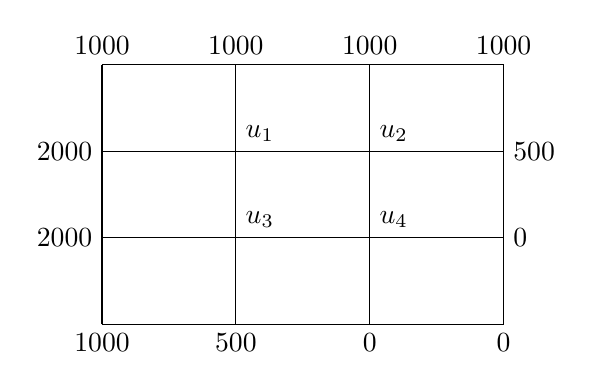
\begin{tikzpicture}[x=1.7cm,y=1.1cm]
 \foreach \i in {0,1,2,3}{\draw (\i,0)--(\i,3); \draw (0,\i)--(3,\i);}
 \foreach \x in {0,1,2,3}{\node[above] at (\x,3) {1000};}
 \node[left] at (0,2) {2000}; \node[left] at (0,1) {2000};
 \node[below] at (0,0) {1000}; \node[below] at (1,0) {500}; \node[below] at (2,0) {0}; \node[below] at (3,0) {0};
 \node[right] at (3,2) {500}; \node[right] at (3,1) {0};
 \node at (1,2) [above right] {$u_1$}; \node at (2,2) [above right] {$u_2$}; \node at (1,1) [above right] {$u_3$}; \node at (2,1) [above right] {$u_4$};
\end{tikzpicture}}}{2}{2}{1}
\qpart{Part -- B}
\q{1a}{Determine the Laplace transform of the periodic function defined by $f(t) = \begin{cases} 1, & 0 \le t < a\\ -1, & a < t \le 2a\end{cases}$ and $f(2a+t) = f(a)$.}{4}{2}{2}
\q{1b}{Express the following function in terms of unit step function and hence obtain its Laplace transform: $f(t) = \begin{cases} t^2, & 1 < t \le 2\\ 4t, & t > 2\end{cases}$.}{6}{3}{3}
\q{2}{Obtain the inverse Laplace transform of the function $F(s) = \dfrac{s}{(s+1)(s^2+1)}$ using the method of partial fractions.}{10}{2}{2}
\q{3}{Employing convolution theorem, determine the inverse Laplace transform of $F(s) = \dfrac{s^2}{s^4-16}$.}{10}{3}{3}
\q{4}{The displacement $x(t)$ of a mass-spring system is governed by $\dfrac{d^2x}{dt^2} + \lambda\dfrac{dx}{dt} + kx = f(t)$, where $\lambda$ and k are force constants subject to the conditions $x(0) = 2$, $\dfrac{dx}{dt}(0) = -4$ and $\lambda = 2$, k = 5, $f(t) = \dfrac{17}{2}\sin 2t$. Determine $x(t)$ by using Laplace transform method.}{10}{--}{4}
\q{5}{Given the values of $u(x,y)$ on the boundary of the square region. Evaluate the function $u(x,y)$ satisfying the Laplace equation $u_{xx}+u_{yy}=0$ at the pivotal points of the figure. Perform four iterations.
\lgrid{60}{60}{60}{60}{0}{40}{50}{30}}{10}{--}{3}
\end{xtable}
\end{xpaper}

% ---------- MA231TB Test II, 20/02/2024
\begin{xpaper}
\paperinfo{deptline={Department of Mathematics},date={20/02/2024},exam={Test II},maxmarks={50},sem={III (AS, BT, CH, IM, ME)},prog={UG},duration={10 AM to 11:30 AM},
 title={Statistics, Laplace Transform and Numerical Methods},code={MA231TB}}
\xhead
\begin{xtable}{Questions}
\q{1a}{By using the convolution theorem evaluate: $\mathcal{L}^{-1}\left[\dfrac{1}{(s+1)s^2}\right]$.}{5}{1}{1}
\q{1b}{Solve $x''(t) + 9x(t) = \cos(2t)$, $x(0) = 1$, $x'(0) = \dfrac{12}{5}$ by method of Laplace transforms.}{5}{3}{2}
\q{2a}{Evaluate: $\mathcal{L}^{-1}\left[\dfrac{s\,e^{-s/2} + \pi e^{-s}}{s^2+\pi^2}\right]$.}{5}{2}{1}
\q{2b}{The equations of regression lines of two variables x and y are $x - y = 0$, $4x - y = 3$ and the standard deviation of x is 1. Obtain the variance of y and the coefficient of correlation between x and y.}{5}{2}{2}
\q{3}{Compute the first four moments about the mean of the frequency distribution given below:
\qtabc{|l|c|c|c|c|c|}{\hline x & 0 & 1 & 2 & 3 & 4\\\hline f & 1 & 8 & 28 & 56 & 70\\\hline}}{10}{2}{3}
\q{4a}{The following table gives ranking of 10 students according to their achievements in both the laboratory and lecture portions of an engineering course. Find the coefficient of rank correlation.
\qtabc{|l|*{10}{c|}}{\hline Lab (x) & 8 & 3 & 9 & 2 & 7 & 10 & 4 & 6 & 1 & 5\\\hline Lecture (y) & 9 & 5 & 10 & 1 & 8 & 7 & 3 & 7 & 2 & 6\\\hline}}{4}{1}{2}
\q{4b}{If the velocity V (km/hr) and the resistance R (kg/tonne) are related by a relation of the form $R = a + bV^2$, find a and b, by the method of least squares, given:
\qtabc{|l|c|c|c|c|c|}{\hline V & 10 & 20 & 30 & 40 & 50\\\hline R & 8 & 10 & 15 & 21 & 30\\\hline}}{6}{3}{1}
\q{5}{The following table shows the weights (z), heights (x) and ages (y) of 8 boys. Find the regression equation of z on x and y, estimate the weight of a boy who is 9 years old and 54 inches tall.
\qtabc{|l|*{9}{c|}}{\hline z (lbs.) & 64 & 71 & 53 & 67 & 55 & 58 & 77 & 57 & \\\hline x (in.) & 57 & 59 & 49 & 62 & 51 & 50 & 55 & 48 & \\\hline y (yrs.) & 8 & 10 & 6 & 11 & 8 & 7 & 10 & 9 & \\\hline}}{10}{3}{4}
\end{xtable}
\end{xpaper}

% ---------- 21MA31C CIE - II, 20/02/2023
\begin{xpaper}
\paperinfo{deptline={Department of Mathematics},date={20/02/2023},exam={CIE -- II},maxmarks={10 + 50},sem={III},prog={BT, CH, CV, IEM, ME},duration={120 Min},
 title={Integral Transforms, Optimization, and Numerical Techniques},code={21MA31C}}
\xhead
\par\noindent{\small\itshape Answer all questions from part A and part B. Part A questions should be answered in the first two pages of the answer book only.}\par\vspace{4pt}
\begin{xtable}{Questions}
\qpart{Part -- A}
\q{01}{The diagonal five-point formula to evaluate $u_{2,2}$ is \blank[1.8cm].}{1}{2}{1}
\q{02}{The partial differential equation $u_{xx} + xu_{yy} = 0$ is classified as \blank[1.8cm].}{1}{1}{2}
\q{03}{For the one-dimensional wave equation $\dfrac{\partial^2u}{\partial t^2} = \dfrac{\partial^2u}{\partial x^2}$ with the boundary conditions $u(0,t) = u(5,t) = 0$, and the initial conditions $u(x,0) = x(x-5)$ and $u_t(x,0) = 0$ with h = 1, k = 1, the value of $u(1,1)$ is \blank[1.8cm].}{2}{2}{2}
\q{04}{The corner points of the feasible region for the objective function z = 3x + 2y subject to the constraints x + 2y $\le$ 10, 3x + y $\le$ 15 and x, y $\ge$ 0 are \blank[1.8cm].}{2}{2}{3}
\q{05}{Write the following L.P.P. in the standard form: Maximize Z = $3x_1 + 2x_2$ subject to $x_1 + 2x_2 \ge 4$, $x_1 - x_2 \le 2$, $2x_1 + 3x_2 = 6$, $x_1, x_2 \ge 0$.}{2}{2}{1}
\q{06}{Determine all the basic solutions of 2x + y + z = 11. Also, identify basic and non-basic variables.}{2}{3}{2}
\qpart{Part -- B}
\q{01}{Given the values of $u(x,y)$ on the boundary of the square region. Evaluate the function $u(x,y)$ satisfying Laplace equation $\nabla^2u = 0$ at the pivotal points of this figure. Perform 6 iterations by Liebman method.
\lgrid{60}{60}{60}{60}{0}{40}{50}{30}}{10}{1}{2}
\q{02}{Determine the values of $u(x,t)$ satisfying the parabolic equation $\dfrac{\partial u}{\partial t} = 4\dfrac{\partial^2u}{\partial x^2}$ and the boundary conditions $u(0,t) = u(8,t) = 0$ and $u(x,0) = 4x - \dfrac{x^2}{2}$ at the points x = i : i = 0, 1, 2, \ldots, 8 and t = $\dfrac{j}{8}$ : j = 0, 1, 2, \ldots, 5.}{10}{3}{1}
\q{03}{The transverse displacement u of a point at a distance x from one end and at any time t of a vibrating string satisfies the equation $16\dfrac{\partial^2u}{\partial x^2} - \dfrac{\partial^2u}{\partial t^2} = 0$, with boundary conditions $u(0,t) = u(5,t) = 0$ and the initial conditions $u(x,0) = \begin{cases} 3x, & 0 \le x \le \frac{5}{2}\\ 20 - 4x, & \frac{5}{2} \le x \le 5\end{cases}$ and $\dfrac{\partial u}{\partial t} = 0$ at t = 0. Solve the equation numerically up to t = 1, taking h = 1 and k = 1/4.}{10}{2}{2}
\q{04}{The temperature distribution $u(x,t)$ is modelled as the one dimensional heat equation $16\dfrac{\partial u}{\partial t} = \dfrac{\partial^2u}{\partial x^2}$, $0 \le x \le 1$, $t > 0$ subject to the boundary conditions $u(0,t) = u(1,t) = 0$, and the initial condition $u(x,0) = 100(x - x^3)$. Determine the temperature distribution $u(x,t)$ by taking $\Delta x = h = \frac{1}{5}$ and $\Delta t = k = \frac{2}{25}$ using Schmidt relation for 5 levels.}{10}{2}{3}
\q{05}{A factory uses three types of machines to produce two types of electronic gadgets. The first gadget requires 12, 4 and 2 hours and the second gadget require 6, 10 and 3 hours respectively on the three types of machines. The total available time in hours on the three machines are 6000, 4000 and 1800. If the two types of gadgets fetch a profit of \rupee 400 and \rupee 1000, formulate the data as a linear programming problem and find the number of gadgets of each type to be produced for getting maximum profit using graphical method.}{10}{3}{4}
\end{xtable}
\end{xpaper}

%%%%%%%%%%%%%%%%%%%%%%%%%%%% WORK SYSTEMS DESIGN
% ---------- IM233AI CIE - II, 2nd December 2024
\begin{iempaper}
\paperinfo{dept={INDUSTRIAL ENGINEERING \& MANAGEMENT},date={2\textsuperscript{nd} December 2024},exam={CIE -- II},maxmarks={10 + 50},sem={III},prog={UG},duration={120 Min},
 title={WORK SYSTEMS DESIGN},code={IM233AI}}
\iemhead
\begin{cietable}{M}{BT}{CO}
\qpart{Part -- A}
\q{1}{List any four techniques of Work Measurement.}{02}{1}{1}
\q{2}{What is meant by the term, ``Muda'' in the context of Lean Manufacturing?}{02}{2}{2}
\q{3}{Distinguish between work element and basic motion element.}{02}{2}{1}
\q{4}{What is the expanded form of MOST?}{02}{1}{3}
\q{5}{Mention the advocate of Toyota Production System.}{02}{1}{2}
\qpart{Part -- B}
\q{1}{Illustrate and explain the pre requisites for determining the valid time standards.}{10}{3}{3}
\q{2}{A time study analyst observed a repetitive work cycle performed by a worker and then studied the task using a predetermined motion time system. During the observation, the analyst made a record of the work elements. He also made a note of worker's performance and rated it as 85\%. Back in the office, the analyst listed the basic motion elements for the task and retrieved from his computer the corresponding normal time values. The sum of normal times for the basic motion elements was 1.38 min. The company uses a PFD allowance factor of 15\%. Determine the standard time for the task.}{10}{3}{3}
\q{3}{The continuous timing method is used to direct time study a manual task cycle consisting of four elements: a, b, c and d. Two parts are produced each cycle. Element d is irregular element performed once in every six cycles. All elements were performance rated at 90\%. The PFD allowance is 11\%. Determine the normalized time for the cycle, standard time per part, the workers efficiency if the worker completes 844 parts in an 8-hour shift during which she works 7 hours and 10 minutes.
\qtabc{|l|c|c|c|c|}{\hline Element & a & b & c & d\\\hline Observed time (min) & 0.35 & 0.60 & 0.86 & 1.46\\\hline}}{10}{4}{3}
\q{4}{Enumerate different categories of Allowances considered in determining the time standards. Present your understanding by providing relevant contexts in which the different categories are applied by organizations in determining standard time.}{10}{4}{1}
\q{5}{Sketch the structure of Lean Production System. Review the key elements of the structure.}{10}{3}{2}
\end{cietable}
\end{iempaper}

% ---------- 21IM33 CIE - II, 22nd February 2023
\begin{iempaper}
\paperinfo{dept={INDUSTRIAL ENGINEERING \& MANAGEMENT},date={22\textsuperscript{nd} February 2023},exam={CIE -- II},maxmarks={10 + 50},sem={III},prog={UG},duration={20 + 90 Min},
 title={WORK SYSTEMS DESIGN},code={21IM33}}
\iemhead
\begin{cietable}{M}{BT}{CO}
\qpart{Part -- A}
\q{1}{Distinguish between snap back and cumulative timing methods.}{02}{2}{3}
\q{2}{According to Taiichi Ohno, the number of waste forms in a manufacturing environment is \blank[1.8cm].}{01}{1}{2}
\q{3}{The meaning of the word Muda in Japanese is \blank[1.8cm].}{01}{1}{2}
\q{4}{Distinguish between accuracy and precision.}{02}{2}{3}
\q{5}{Distinguish between First generation and Higher generation levels of PMTS.}{02}{2}{3}
\q{6}{List the five steps in the direct time study procedure.}{02}{1}{3}
\qpart{Part -- B}
\q{1}{Classify and explain briefly different methods used to determine the time standards.}{10}{3}{3}
\q{2}{What is a Work Element? Mention at least six guidelines for defining work elements in direct time study. Supplement with appropriate explanation and examples.}{10}{3}{3}
\q{3}{The continuous timing method in direct time study was used to obtain the elemental times for a worker machine task as indicated. Element c is a machine controlled and the time is constant. Elements a, b, d, e and f are operator controlled and external to machine cycle and they are performance rated at 80\%. If the machine allowance is 25\% and worker PFD allowance is 15\%, determine the normal time and standard time for the work cycle.
\qtabc{|l|c|c|c|c|c|c|}{\hline Element & a & b & c & d & e & f\\\hline Observed Time (min) & 0.18 & 0.30 & 0.88 & 1.12 & 1.55 & 1.80\\\hline}}{10}{3}{3}
\q{4}{Enumerate the three activity sequence models in Basic MOST with suitable examples.}{10}{4}{3}
\q{5}{Illustrate the structure of Lean Production System. Explain the features of different elements of the structure.}{10}{3}{2}
\end{cietable}
\end{iempaper}

% ---------- 18IM35 CIE - II, October 2019
\begin{xpaper}
\paperinfo{deptline={Department of Industrial Engineering and Management},date={October 2019},exam={CIE -- II},maxmarks={60},sem={III},prog={UG},duration={90 Min},
 title={Work Systems Design},code={18IM35},note={Use of t distribution tables permitted.}}
\xhead
\begin{xtable}{Questions}
\qpart{Part -- A (Max. Marks 10)}
\q{1.1}{Distinguish between the terms ``Accuracy'' and ``Precision''.}{2}{2}{1}
\q{1.2}{List the four prerequisites for valid time standards.}{2}{1}{3}
\q{1.3}{The standard time is referred to as allowed time. Justify.}{2}{3}{3}
\q{1.4}{The evaluation of the workers performance is \blank[1.8cm].}{1}{1}{3}
\q{1.5}{The time units in MTM are called as \blank[1.8cm].}{1}{1}{4}
\q{1.6}{The motion aggregates in Basic MOST are called as \blank[1.8cm].}{1}{1}{4}
\q{1.7}{What is the meaning of `Coverage' in the application of Standard Data System?}{1}{2}{4}
\qpart{Part -- B (Max. Marks 50)}
\q{1}{The observed element times and performance ratings collected in a direct time study are indicated in the table below. The snapback timing method was used. The PFD allowance in the plant is 14\%. All elements are regular elements in the work cycle. Determine (a) the normal time and (b) the standard time for the cycle.
\qtabc{|l|c|c|c|c|}{\hline Work element & a & b & c & d\\\hline Observed time (min) & 0.22 & 0.41 & 0.30 & 0.37\\\hline Performance ratings (\%) & 90 & 120 & 100 & 90\\\hline}}{10}{3}{3}
\q{2}{The snapback timing method was used to obtain average times for work elements in one work cycle. The times are given in the table below. Element d is a machine-controlled element and the time is constant. Element a, b, c, e and f are operator-controlled and were performance rated at 80\%; however, elements e and f are performed during the machine controlled element. The machine allowance is zero (no extra time is added to the machine cycle), and the PFD allowance is 14\%. Determine (a) the normal time for the cycle and (b) the standard time for the cycle.
\qtabc{|l|c|c|c|c|c|c|}{\hline Element & a & b & c & d & e & f\\\hline Observed time (min) & 0.24 & 0.30 & 0.17 & 0.76 & 0.26 & 0.14\\\hline}}{10}{4}{3}
\q{3a}{Seven cycles have been observed during a direct time study. The mean for the largest element time is 0.85 min, and the corresponding sample standard deviation s is 0.15 min, which was also the largest. If the analyst wants to be 95\% confident that the mean of the sample was within $\pm$0.10\% of the true mean, how many more observations should be taken?}{05}{3}{3}
\q{3b}{Review the key features of MOST.}{05}{2}{4}
\q{4}{Illustrate the classification of methods to determine time standards. Explain any two of them in detail.}{10}{3}{2}
\q{5}{Elaborate the procedure in determining time standard using the technique of Predetermined Motion Time Systems (PMTS).}{10}{2}{3}
\end{xtable}
\end{xpaper}

%%%%%%%%%%%%%%%%%%%%%%%%%%%% MANUFACTURING PROCESSES
% ---------- IM234AI CIE - II, 3rd December 2024
\begin{iempaper}
\paperinfo{dept={INDUSTRIAL ENGINEERING \& MANAGEMENT},date={3\textsuperscript{rd} December 2024},exam={CIE -- II},maxmarks={10 + 50},sem={III},prog={UG},duration={120 Min},
 title={MANUFACTURING PROCESSES},code={IM234AI}}
\iemhead
\begin{cietable}{M}{BT}{CO}
\qpart{Part -- A}
\q{1}{The \blank[1.8cm] is the sharp edge at the point where the side cutting edge and end cutting edge meet.}{1}{2}{2}
\q{2}{A common defect in arc welding is \blank[1.8cm], which occurs when the arc is unstable and leads to uneven welding.}{1}{2}{3}
\q{3}{The \blank[1.8cm] casting process involves using a permanent metal mold and injecting molten metal under high pressure to create parts.}{1}{2}{2}
\q{4}{The \blank[1.8cm] of a single-point tool is the angle formed between the flank of the tool and the workpiece surface, which helps in controlling the chip flow.}{1}{1}{1}
\q{5}{List any two applications of shell molding process.}{2}{2}{2}
\q{6}{List any two advantages of centrifugal casting.}{2}{1}{2}
\q{7}{State any two difference between orthogonal and oblique cutting.}{2}{1}{3}
\qpart{Part -- B}
\q{1}{With a neat sketch explain the casting process which is best suited for casting of hollow pipes and tubes.}{10}{2}{1}
\q{2}{With the help of neat sketch, explain the working principle of Projection Welding.}{10}{1}{2}
\q{3}{Explain the working principle of the welding process that uses a focused beam of high-velocity electrons to generate heat for melting and fusing materials, particularly in applications requiring precision, such as aerospace, automotive, and electronics manufacturing?}{10}{3}{3}
\q{4}{Describe the working principle of the casting method that uses a wax pattern coated with a ceramic shell to create a mold, which is then used to produce highly detailed and complex components for applications such as aerospace turbine blades, medical implants, and precision automotive parts?}{10}{3}{2}
\q{5}{What are the different types of chips that are formed in metal machining and give the conditions that are favorable to their formation?}{10}{2}{3}
\end{cietable}
\end{iempaper}

% ---------- IM234AI CIE - II, 22nd February 2024
\begin{iempaper}
\paperinfo{dept={INDUSTRIAL ENGINEERING \& MANAGEMENT},date={22\textsuperscript{nd} February 2024},exam={CIE -- II},maxmarks={50},sem={III},prog={UG},duration={90 Min},
 title={MANUFACTURING PROCESS},code={IM234AI}}
\iemhead
\begin{cietable}{M}{BT}{CO}
\q{1}{Enumerate the importance of pattern making and discuss different types of pattern making materials.}{10}{1}{1}
\q{2}{List and discuss the essential properties required for a moulding sand.}{10}{2}{2}
\q{3}{Classify and explain the basic bulk forming process with a neat sketch.}{10}{3}{3}
\q{4}{Discuss the importance of roll presses with the following:
\begin{rom}\item Breakdown Passes\item Roughing Passes\item Finishing Passes\end{rom}}{10}{2}{2}
\q{5}{Differentiate with a neat sketch, between direct and indirect extrusion with the reference to following:
\begin{rom}\item Material flow\item Force required\item Another name\item Material wastages\item Frictional force\end{rom}}{10}{3}{3}
\end{cietable}
\end{iempaper}

% ---------- 18IM36 CIE - II, October 2019
\begin{xpaper}
\paperinfo{deptline={Department of Industrial Engineering and Management},date={October 2019},exam={CIE -- II},maxmarks={60},sem={III},prog={UG},duration={120 Min},
 title={Manufacturing Process},code={18IM36}}
\xhead
\begin{xtable}{Questions}
\qpart{Part -- A (Max. Marks 10)}
\q{1}{During milling operation cutter moves \blank[1.8cm] to its axis.}{(01)}{1}{1}
\q{2}{An arbor is used hold the milling \blank[1.8cm].}{(01)}{1}{1}
\q{3}{In a milling operation, length of the cut is 360 mm and feed rate is 180 mm/min, then milling time in minutes is \blank[1.8cm].}{(01)}{1}{1}
\q{4}{The use of coatings on milling cutters will increase the \blank[1.8cm] hardness of the tool.}{(01)}{1}{1}
\q{5}{Gang milling refers to the use of two or more milling cutters mounted on the arbor in a \blank[1.8cm] milling set up.}{(01)}{1}{1}
\q{6}{Cutting T-slots can be performed more effectively by \blank[1.8cm] milling machine.}{(01)}{1}{1}
\q{7}{The dividing heads are of \blank[1.8cm] types.}{(01)}{1}{1}
\q{8}{By linking the worm and worm gear driving mechanism of the attachment with the leadscrew of the table, continuous \blank[1.8cm] motion can be imparted to the workpiece.}{(01)}{1}{1}
\q{9}{If drill is 5.5 mm, metal removal rate is 65 mm3/minute and rpm is 130. Then \blank[1.8cm] is value of feed in mm/revolution.}{(01)}{2}{2}
\q{10}{If t = 2 minute, n = 2 rpm and s = 5 mm. t = machining time in minute, l = length of travel of the drill in mm, n = rpm of the drill and s = feed per revolution of the drill in mm. Then \blank[1.8cm] is the value of l.}{(01)}{2}{2}
\qpart{Part -- B (Max. Marks 50)}
\q{1}{Explain the nomenclature of a milling cutter with a neat sketch.}{(10)}{1}{1}
\q{2}{Differentiate between up milling \& down milling with respect to the following: (i) Sketch (ii) Alternate name (iii) Chip thickness (iv) Job lifting tendency (v) Practicability.}{(10)}{1}{1}
\q{3}{Discuss with a neat sketch the geometry of twist drill.}{(10)}{1}{1}
\q{4}{State clearly, the Plate No. and the indexing movements to be made using a Universal dividing head, to divide the periphery of a work into 69 equal divisions. Following indexing plates are available: Plate No. 1: 15, 16, 17, 18, 19, 20; Plate No. 2: 21, 23, 27, 29, 31, 33; Plate No. 3: 37, 38, 41, 43, 47, 49.}{(10)}{2}{2}
\q{5}{A hole with 40 mm diameter and 50 mm depth is to be drilled in mild steel component. The cutting speed can be taken as 65 m/min and feed rate as 0.25 mm/rev. Calculate the machining time and the metal removal rate.}{(10)}{--}{--}
\end{xtable}
\end{xpaper}

%%%%%%%%%%%%%%%%%%%%%%%%%%%% DIGITAL METROLOGY
% ---------- IM235AI CIE - II, 4th December 2024
\begin{iempaper}
\paperinfo{dept={INDUSTRIAL ENGINEERING \& MANAGEMENT},date={4\textsuperscript{th} December 2024},exam={CIE -- II},maxmarks={10 + 50},sem={III},prog={UG},duration={120 Min},
 title={DIGITAL METROLOGY},code={IM235AI}}
\iemhead
\begin{cietable}{M}{BT}{CO}
\qpart{Part -- A}
\q{1}{List the Basic components used in ADCs and DACs.}{02}{1}{2}
\q{2}{Mention the principle of working of Piezoelectric sensor.}{01}{2}{2}
\q{3}{Distinguish between Unilateral and Bilateral Tolerance.}{02}{2}{3}
\q{4}{How a Feature Control Frame represented in a GD\&T technical drawing?}{01}{1}{3}
\q{5}{Differentiate between allowance and clearance?}{02}{2}{3}
\q{6}{What is Interchangeability?}{02}{2}{3}
\qpart{Part -- B}
\q{1}{Evaluate the operational mechanisms of tactile sensors critically analyzing their fundamental principles and contact detection capabilities. Provide examples of applications where these sensors are commonly used.}{10}{3}{2}
\q{2}{Determine the actual dimension to be provided for a shaft and hole of 70 mm size for F$_8$e$_9$ type of fit.
\begin{rom}\item Size 70 mm falls in the diameter step of 50 mm -- 80 mm.\item Value of tolerances for IT8 and IT9 are 25i and 40i.\item Value of fundamental deviation for `F' type shaft is 5.5D$^{0.41}$ and for `e' type shaft is $-$11D$^{0.41}$.\end{rom}
Calculate the maximum and minimum clearance. Also mention the type of fit. Represent the dimensions graphically.}{10}{4}{3}
\q{3}{Discuss the different types of fits commonly used in engineering assemblies. Explain the characteristics, advantages, and applications of each type of fit, illustrating your answer with relevant examples.}{10}{3}{3}
\q{4}{Write a note Upper deviation and Lower deviation and Fundamental deviation. Describe the concepts of the hole basis system and shaft basis system in engineering fits. Explain how these systems are implemented in manufacturing processes and their significance in ensuring functional compatibility and quality of assembled parts.}{10}{2}{3}
\q{5}{Write a note on the following and represent schematically. Basic Hole, Basic Shaft, Minimum Limit of Size, Maximum clearance, Minimum Clearance.}{10}{2}{3}
\end{cietable}
\end{iempaper}

% ---------- IM235AI CIE - II, 24th February 2024
\begin{iempaper}
\paperinfo{dept={INDUSTRIAL ENGINEERING \& MANAGEMENT},date={24\textsuperscript{th} February 2024},exam={CIE -- II},maxmarks={50},sem={III},prog={UG},duration={90 Min},
 title={DIGITAL METROLOGY},code={IM235AI}}
\iemhead
\begin{cietable}{M}{BT}{CO}
\q{1.}{Explain the principle of Interference and Describe with neat sketches the working of an autocollimator. Explain how these tools are used in manufacturing processes for measurement of straightness.}{10}{3}{3}
\q{2.}{Define Crest, Flank and Pitch and schematically represent on a screw thread. Explain how the major diameter of a screw thread can be measured using Bench micrometer.}{10}{3}{3}
\q{3.}{Determine the actual dimension to be provided for a shaft and hole of 90 mm size for h$_8$E$_9$ type of fit.
\begin{rom}\item Size 90 mm falls in the diameter step of 80 mm--100 mm.\item Value of tolerances for IT8 and IT9 are 25i and 40i.\item Value of fundamental deviation for `e' type shaft is 11D$^{0.41}$.\end{rom}
Also mention the type of fit. Represent the dimensions graphically.}{10}{4}{2}
\q{4.}{Define Upper deviation and Lower deviation and Fundamental deviation. Describe the concepts of the hole basis system and shaft basis system in engineering fits. Explain how these systems are implemented in manufacturing processes and their significance in ensuring functional compatibility and quality of assembled parts.}{10}{2}{2}
\q{5.}{Discuss different types of surface finish analysis techniques and irregularities commonly encountered in engineering. Explain the significance of surface finish analysis in manufacturing processes, and how identifying irregularities contributes to product quality and performance. Provide examples to support your explanation.}{10}{3}{3}
\end{cietable}
\end{iempaper}

% ---------- 18IM34 CIE - II, October 2019
\begin{xpaper}
\paperinfo{deptline={Department of Industrial Engineering and Management},date={October 2019},exam={CIE -- II},maxmarks={60},sem={III},prog={UG},duration={120 Min},
 title={Metrology and Measurements},code={18IM34}}
\xhead
\begin{xtable}{Questions}
\qpart{Part -- A}
\q{1.1}{\blank[1.8cm] is a new standard in communication used in CAM.}{(01)}{L2}{CO3}
\q{1.2}{\blank[1.8cm] is the sensory part of a CMM responsible for sensing different parameters required for measurement.}{(01)}{L1}{CO3}
\q{1.3}{The data-collecting unit in a CMM is the \blank[1.8cm].}{(01)}{L1}{CO3}
\q{1.4}{A pointed instrument used as an input device in the probe of a CMM is \blank[1.8cm].}{(01)}{L1}{CO3}
\q{1.5}{List the different types of gauges according to the form of testing surface.}{(01)}{L1}{CO2}
\q{1.6}{List any two considerations in the selection of gauge material.}{(01)}{L1}{CO2}
\q{1.7}{Wear allowance is provided on the \blank[1.8cm] side of the gauge.}{(01)}{L1}{CO2}
\q{1.8}{`GO' Limit refers to \blank[1.8cm].}{(01)}{L1}{CO2}
\q{1.9}{The Optical flat is made up of \blank[1.8cm] material.}{(01)}{L2}{CO2}
\q{1.10}{Type B Optical Flat is used for \blank[1.8cm].}{(01)}{L2}{CO3}
\qpart{Part -- B}
\q{Q1}{Design the `General' type `GO' and `NOGO' gauges for the components having 50H8c8 fit. Given the following with usual notations: (i) Upper deviation for Shaft = (95 + 0.8D) microns (ii) 50 mm falls in the diameter step of 50--80 mm (iii) IT8 = 25i. Take wear allowance as 10\% of the gauge Tolerance. Also mention the type of fit. Represent the dimensions graphically.}{(10)}{--}{--}
\q{Q2}{Enumerate on the different types of Main structure of a Coordinate Measuring Machine with neat sketches, and list out the industrial Applications of a CMM.}{(10)}{--}{--}
\q{Q3a}{Describe the role of CMM in Computer Aided Manufacturing.}{(06)}{--}{--}
\q{Q3b}{Explain briefly the advantages of CMM.}{(04)}{--}{--}
\q{Q4}{Describe briefly the Inductive and Optical Transmission Probes with neat sketches.}{(10)}{--}{--}
\q{Q5a}{Explain briefly the Taylor's principle of gauge design with neat sketches.}{(06)}{--}{--}
\q{Q5b}{Enumerate on the Allocation of Tolerance on Gauge Design.}{(04)}{--}{--}
\end{xtable}
\end{xpaper}

%%%%%%%%%%%%%%%%%%%%%%%%%%%% MECHANICS OF MATERIALS
% ---------- 21IM32 CIE - II, 21st February 2023
\begin{iempaper}
\paperinfo{dept={INDUSTRIAL ENGINEERING AND MANAGEMENT},date={21\textsuperscript{st} February 2023},exam={CIE -- II},maxmarks={10 + 50},sem={III},prog={UG},duration={20 + 90 Min},
 title={MECHANICS OF MATERIALS},code={21IM32}}
\iemhead
\begin{cietable}{M}{BT}{CO}
\qpart{Part -- A}
\q{1}{The number of phases present in Equilibrium at Eutectic point is \blank[1.8cm].}{1}{3}{1}
\q{2}{What reaction does this equation denote? Liquid + Solid1 $\to$ Solid 2}{1}{2}{2}
\q{3}{Expand T T T Diagram?}{1}{2}{3}
\q{4}{What is the triple point of water?}{2}{2}{1}
\q{5}{Enumerate Gibb's Phase rule?}{2}{3}{3}
\q{6}{$\alpha$-ferrite has a \blank[1.8cm] crystal structure.}{1}{2}{2}
\q{7}{What is the composition of Carbon at cementite?}{1}{2}{3}
\q{8}{For a circular shaft of diameter subjected to torque the maximum value of the shear stress is \blank[1.8cm].}{1}{2}{2}
\qpart{Part -- B}
\q{1}{Derive Torsion Equation with a neat diagram.}{10}{3}{2}
\q{2}{Draw Fe-Fe3C diagram and differentiate between cementite, austrinite and ferrite.}{10}{2}{3}
\q{3}{A solid shaft rotating at 500 rpm transmits 30 KW. Max torque is 20\% more than the mean torque. Material of the shaft has an allowable shear stress 65 MPa and modulus of rigidity 81 GPa. Angle of twist in the shaft should not exceed 1$^{\circ}$ per meter length of shaft. Determine the safe diameter of shaft.}{10}{2}{3}
\q{4}{Two metals Al and Cu have melting point at 800 $^{\circ}$C and 500 $^{\circ}$C. The alloy pair forms eutectic at 400 $^{\circ}$C of compositions 60\% Al and 40\% Cu, the solid solubilities are as follows: 20\% Cu in Al at 400 $^{\circ}$C and 10\% Cu in Al at 0 $^{\circ}$C; 10\% Al in Cu at 400 $^{\circ}$C and 5\% Al in Cu at 0 $^{\circ}$C. Assume the liquidus, solidus and solvent lines to be straight, no solid state reaction in the series.
\begin{rom}\item Draw the phase diagram for the series and label all the salient temperature, composition and regions.\item Find the amount of solid and liquid present at 450 $^{\circ}$C.\end{rom}}{10}{2}{1}
\q{5}{Explain using cooling curves, how the Binary phase diagram are constructed?}{10}{3}{4}
\end{cietable}
\end{iempaper}

%%%%%%%%%%%%%%%%%%%%%%%%%%%% BASKET / OTHER-DEPARTMENT COURSES
% ---------- ME232TB Material Science for Engineers, CIE - II, 3rd December 2024
\begin{xpaper}
\paperinfo{deptline={Department of Mechanical Engineering},date={3\textsuperscript{rd} December 2024},exam={CIE -- II},maxmarks={50 + 10},sem={III},prog={UG},duration={120 Min},
 title={Material Science for Engineers},code={ME232TB}}
\xhead
\begin{xtable}{Questions}
\qpart{Part A (Quiz)}
\q{1.}{Semiconductor device with a p-n junction which produces current by absorption of light in the depletion region is termed as \blank[1.8cm].}{1}{1}{2}
\q{2.}{\blank[1.8cm] is the metal joining process in which parent metal pieces are heated either to plastic or molten state.}{1}{1}{2}
\q{3.}{If the emission of radiation occurs longer than 10$^{-8}$ seconds is known as \blank[1.8cm].}{1}{1}{2}
\q{4.}{Alloying elements of HSS are \blank[1.8cm].}{1}{1}{2}
\q{5.}{Lightest of commonly used metals is \blank[1.8cm].}{1}{1}{2}
\q{6.}{Define young's modulus of a material with equation.}{2}{2}{2}
\q{7.}{\blank[1.8cm] is the type of glass that cannot allow heat through it because of air between the layers and acts as good insulators.}{1}{1}{2}
\q{8.}{Concrete is a composite material made up of \blank[1.8cm] and \blank[1.8cm].}{2}{1}{2}
\qpart{Part B (Test)}
\q{1a}{What is piezoelectric effect? Explain the applications of piezoelectric materials.}{05}{2}{2}
\q{1b}{Distinguish between ductile and brittle fracture.}{05}{2}{2}
\q{2}{With the stress strain diagram explain the mechanical properties of a ductile metal.}{10}{2}{2}
\q{3a}{Discuss the applications of semiconductors.}{05}{3}{2}
\q{3b}{Explain four different types of cast iron based on microstructure, properties and applications.}{05}{2}{2}
\q{4a}{With a neat sketch describe the steps to be followed in metal casting process.}{05}{2}{2}
\q{4b}{Compare thermoplastics with thermosetting plastics.}{05}{3}{2}
\q{5a}{Justify the need for composite materials. Classify composite materials.}{05}{3}{2}
\q{5b}{What is a biomaterial? List the desirable properties of biomaterials.}{05}{2}{2}
\end{xtable}
\end{xpaper}

% ---------- ME232AT Materials Science for Engineers, CIE II, 20th February 2024
\begin{xpaper}
\paperinfo{deptline={Department of Mechanical Engineering},date={20\textsuperscript{th} February 2024},exam={CIE -- II},maxmarks={50},sem={3},prog={UG},duration={90 Minutes},
 title={Materials Science for Engineers},code={ME232AT}}
\xhead
\begin{xtable}{Questions}
\q{1a.}{With the help of a stress-strain diagram explain toughness and ductility of a material.}{04}{3}{2}
\q{1b.}{Using stress-strain diagram distinguish ductile and brittle fracture.}{06}{2}{2}
\q{2.}{Explain the following properties: thermal expansion coefficient, thermocouple, luminescence, optical fibres.}{10}{3}{2}
\q{3.}{Describe the following: ferroelectricity, piezoelectricity, superconductor.}{10}{4}{2}
\q{4.}{Explain the properties and applications of following materials with examples. Ceramics and Fiber reinforced composites.}{10}{3}{2}
\q{5.}{Explain the properties and applications of following materials: stainless steel, cast iron and titanium alloys.}{10}{3}{2}
\end{xtable}
\end{xpaper}

% ---------- CV232AT Environment and Sustainability, CIE - II (Quiz + Test), 3/12/2024
\begin{xpaper}
\paperinfo{deptline={Department of Civil Engineering},date={3/12/2024},exam={CIE -- II (Quiz + Test)},maxmarks={60},sem={III},prog={UG},duration={90 Min + 20 Min},
 title={Environment and Sustainability (Basket Course)},code={CV232AT}}
\xhead
\begin{xtable}{Questions}
\qpart{Part A}
\q{1.}{Describe the term of ``environmental audit''?}{1}{1}{2}
\q{2.}{Explain the need for new energy sources.}{1}{2}{3}
\q{3.}{Classify different types of energy sources.}{1}{2}{3}
\q{4.}{Differentiate between linear and cyclical resource management systems.}{1}{2}{3}
\q{5.}{Describe the working principle of tidal energy converter in renewable energy generation.}{2}{1}{2}
\q{6.}{State the significance of GDP in environmental economics.}{2}{1}{2}
\q{7.}{Enumerate the importance of environmental economics.}{2}{2}{3}
\qpart{Part B}
\q{1a.}{Illustrate carbon cycle with sketch.}{05}{2}{2}
\q{1b.}{What are the advantages of hydrogen energy?}{05}{2}{2}
\q{2.}{Describe ocean thermal energy conversion with its advantages and limitations.}{10}{2}{2}
\q{3.}{Enumerate the concept of sustainable urbanization and the need for the same.}{10}{2}{3}
\q{4a.}{Discuss the steps in environmental audit.}{05}{2}{3}
\q{4b.}{Enumerate the economics and social aspects of sustainability.}{05}{2}{3}
\q{5.}{Illustrate the concept of economics and its integration to social aspects for sustainability.}{10}{2}{3}
\end{xtable}
\end{xpaper}

% ---------- CV232AT Environment and Sustainability, CIE - II (Test), 20-02-2024
\begin{xpaper}
\paperinfo{deptline={Department of Civil Engineering},date={20-02-2024},exam={CIE -- II (Test)},maxmarks={50},sem={III (Basket Course)},prog={UG},duration={90 Min},
 title={Environment and Sustainability},code={CV232AT}}
\xhead
\begin{xtable}{Questions}
\q{1.}{Enumerate the process of energy management and energy conservation with its objectives.}{10}{2}{3}
\q{2.}{Explain any 5 types of alternate energy sources with their advantages and disadvantages.}{10}{3}{1}
\q{3.}{Enumerate the objectives of sustainable urban projects.}{10}{2}{3}
\q{4.}{Highlight five important principles of sustainable development.}{10}{3}{3}
\q{5a.}{Briefly explain any 5 international protocols and agreements that address specific environmental issues.}{05}{2}{2}
\q{5b.}{Describe any 5 disadvantages of linear resource management systems.}{05}{3}{2}
\end{xtable}
\end{xpaper}

% ---------- BT232AT Bio Safety Standards and Ethics, Quiz and Test - 2, December 3, 2024
\begin{xpaper}
\paperinfo{deptline={Department of Biotechnology},date={December 3, 2024},exam={Closed Book Offline Quiz and Test -- 2},maxmarks={10 + 50},sem={III},prog={UG},duration={120 Min},
 title={Bio Safety Standards and Ethics (Basket Course)},code={BT232AT}}
\xhead
\begin{xtable}{Questions}
\qpart{Part A}
\q{1}{A passenger in flight found a bolt and nut in the burger. Identify the type of the hazard.}{1}{2}{3}
\q{2}{Expand the term GMP.}{1}{2}{4}
\q{3}{Name any one food certification followed in the world.}{1}{2}{3}
\q{4}{Expand the term GHP.}{1}{2}{4}
\q{5}{A person found a frog leg in the food. Identify the type of the hazard.}{1}{2}{4}
\q{6}{\blank[1.8cm] types of licences issued by FSSAI.}{1}{2}{3}
\q{7}{Name two diseases caused due to food contamination.}{1}{2}{4}
\q{8}{Milk is heated to \blank[1.8cm] $^{\circ}$C temperature during pasteurization.}{1}{1}{3}
\q{9}{What is 2-hour 4-hour rule for food storage.}{2}{2}{3}
\qpart{Part B (Test)}
\q{1}{Define food contamination. Mention and explain with examples the types of Hazard which contaminate food.}{10}{2}{3}
\q{2}{Elaborate on the basic rules of hygiene, sanitation and safety in food processing.}{10}{3}{3}
\q{3}{Explain in detail how to eliminate the different type of hazards which contaminate food.}{10}{3}{3}
\q{4a}{Mention the principles of HACCP.}{5}{3}{4}
\q{4b}{Decode the FSSAI license number 20719078324011 (Lic. No. as printed on the FSSAI logo).}{5}{2}{3}
\q{5a}{Explain in detail the instruments used in food testing laboratory.}{5}{3}{4}
\q{5b}{Illustrate the various analytical methods used in food testing process.}{5}{3}{4}
\end{xtable}
\end{xpaper}

\end{document}
